\documentclass[a4paper,12pt]{article}
\usepackage[T2A]{fontenc}    
\usepackage[utf8]{inputenc}  % зависит от кодировки Вашего документа
\usepackage[english,russian]{babel}
\usepackage{graphicx}
\usepackage{ragged2e}
\usepackage{amsmath}
\usepackage{algorithm}
\usepackage{algpseudocode}
\usepackage{array}
\usepackage{tabularx}
\usepackage{comment}
\usepackage[letterpaper,left=30mm,right=15mm,bottom=25mm,top=25mm]{geometry}
\usepackage{indentfirst}
\setlength{\parindent}{1.25cm}
\setlength{\parskip}{0cm}

\usepackage{titlesec}

\usepackage{color}

\usepackage{setspace}

\linespread{1.5}

\usepackage{titlesec}

\usepackage[hidelinks]{hyperref}


\usepackage{amssymb,amsfonts,amsmath,amsthm} % математические дополнения от АМС
\usepackage{cleveref}
\usepackage{graphicx}
\usepackage{float}
\usepackage{caption}
\usepackage{subcaption}
\usepackage{epstopdf}

\begin{document}
\begin{titlepage}
		
	\begin{spacing}{1.}
	\begin{center}
	    \large \bfseries
	    Федеральное государственное бюджетное образовательное\\
	    учреждение высшего образования\\ 
        Московский государственный университет\\
        имени М.В. Ломоносова
	\end{center}
	
	\begin{center}
	    \large \bfseries
	    Казахстанский филиал\\ 
        Направление 01.03.02 «Прикладная математика и \\
        информатика»
	\end{center}
	
	\vspace{5\baselineskip}
	\begin{center}
	    \large Селевенко Роман Михайлович
	\end{center}
	
	\vspace{1\baselineskip}
	\begin{center}
	    \large \bfseries
	    Об алгоритме поиска древесной ширины графов
	\end{center}
	
	\vspace{1\baselineskip}
	\begin{center}
	    \large Выпускная квалификационная работа
	\end{center}
	
	\vspace{4\baselineskip}
	\begin{flushright}
	    \textbf{Научный руководитель:} \\старший преподаватель \\
	    профессор, д.ф.-м.н. С.Н.Селезнева\\
	    \textbf{Допустить к защите:} \\
	    и.о. заведующего кафедрой\\
	    Л.В. Крицков\\
	\end{flushright}
	
	\begin{flushright}
	    \makebox[4.5cm]{\hrulefill}\\
	    (подпись и.о. зав. кафедрой)
	\end{flushright}
	
	\vspace{1\baselineskip}
	\begin{flushright}
	    «\makebox[1.5cm]{\hrulefill}» \makebox[4cm]{\hrulefill} 2022 г.
	\end{flushright}
	
	\vspace{3\baselineskip}
	\begin{center}
	    \bfseries
	    Нур-Султан, 2022
	\end{center}
	
	\end{spacing}
\end{titlepage}
	
                                                                        

		\clearpage
		\tableofcontents
		\clearpage
    
		\newpage
		\section{Введение}
		\renewcommand{\baselinestretch}{1.5}
		\begin{large}

		В этой работе рассматриваются алгоритмы получения древесной ширины графа и основные свойства древесной ширины графов.
		
		Эти алгоритмы могут быть полезны в сферах искусственного интеллекта, исследования операций и многих других.

		Древесная ширина — это минимальная ширина среди всех древесных разложений графа. Под древесным разложением графа понимают его представление в виде дерева с узлами, которые являются множествами вершин исходного графа с определенными свойствами.
		В начале 70-х было обнаружено, что для огромного количества оптимизационных задач на графах сложность алгоритмов может быть уменьшена с помощью динамического программирования, если граф имеет ограниченную величину, которая в [1] соответствует древесной ширине.

		Позже, в конце 80-х, несколько авторов [2, 3, 4] обнаружили, что некоторое количество NP-полных задач для случайных графов могут быть решены более эффективно для графов с ограниченной древесной шириной, используя древесные декомпозиции этих графов. 
		К примеру, задача раскраски графа древесной ширины k в k цветов может быть решена алгоритмом динамического программирования на древесной декомпозиции графа.
		Для каждого множества в древесной декомпозиции графа и каждого разбиения в этом множестве на цвета, алгоритм определяет, является ли эта раскраска допустимой и можно ли ее расширить.
		Алгоритм находит оптимальную раскраску со сложностью $O(k(k+n))$, где $n$ — это количество вершин в графе.
		В 1987 году показано, что задача о том, больше ли древесная ширина числа $k$, — NP-полна [5].
		Однако, существует полиномиальный алгоритм отвечающий на вопрос, имеет ли данный граф древесную ширину меньшую чем $k$, где $k$ — постоянная величина [6].

		Графы с небольшой древесной шириной, вследствие малого количества элементов в вершинах древесной декомпозиции могут быть пройдены быстрее чем графы с большой древесной шириной.
		Известно что, граф с древесной шириной 1 это дерево, граф с древесной шириной 2 это параллельно-последовательный граф, граф с древесной шириной 3 --- граф Халина [7].

		В связи обширным применением древесной ширины, существует большое количество алгоритмов находящих её. 
		Рассмотрим сначала точные алгоритмы нахождения древесной ширины.
		Пусть $k$ — древесная ширина, $n$ — количество вершин в графе $G$, $m$ — количество ребер в графе $G$.
		В 1987 году получен алгоритм [8] определяющий, является ли текущий граф k-деревом со сложностью $O(n^{(k+2)})$.
		В работе 1995 года [9] получен алгоритм решающий проблему нахождения декомпозиции графа на ветви (а следовательно, и древесной декомпозиции) со сложностью $O((n+1)^2 + m + n + 1)$.

		Также существуют алгоритмы оценивающие древесную ширину сверху.
		Алгоритм из работы 1996 года [10] оценивает древесную ширину за линейное время $O(n)$.
		Этот линейный алгоритм для постоянного $k$, которому дан граф $G$, определяет больше ли древесная ширина этого графа числа $k$, и если это так, находит древесную декомпозицию $G$ с древесной шириной не больше $k$.
		Алгоритм из работы [11] который имеет оценку сложности $O(k\sqrt{(\log{k})})$ основан на связи между древесной шириной и максимальным сепаратором. Данный алгоритм работает за полиномиальное время $O(n^2)$.
		Следующий алгоритм нахождения древесной ширины графов --- алгоритм изложенный в [12].
		В этой статье для $k \leq 3$ было доказано существование линейного вероятностного алгоритма определяющего имеет ли граф $G$ древесную ширину $\leq k$.
		Алгоритм имеет сложность $O(n\log^2{n}+n\log{n}|\log{p}|)$.
		Также можно зафиксировать величину $k$ и определить является ли это значение рёбер древесной шириной графа. 
		Например, в работе [13] авторы используют утверждение, что граф $G$ с $n$ вершинами может быть приведен к нуль-графу с $n$ вершинами тогда и только тогда, когда он явлется подграфом 3-дерева. 
		Здесь был получен полиномильный алгоритм со сложностью ($O(n\log{n})$) для определения того, является ли граф частичным 3-деревом и для нахождения вложения в 3-дереве, если такое вложение существует.
		
		В этой работе мы рассмотрим жадный алгоритм, оценивающий сверху древесную ширину.

		\end{large}

		\newpage
		\section{Основные определения}
		\renewcommand{\baselinestretch}{1.5}
		\begin{large}
		Введем основные определения и обозначения(см. например,  [14, 15])

		Пусть $V$ --- непустое множество, $V^{(2)}$ --- множество всех его двухэлементных подмножеств.
		Пара $(V,E)$, где $E$ --- произвольное подмножество множества $V^{(2)}$, называется {\it графом} ({\it неориентированным графом}). 
		Элементы множества $V$ называются {\it вершинами} графа, а элементы множества $E$ {\it ребрами}.
		Множества вершин и ребер графа $G$ обозначаются $V(G)$ и $E(G)$ соответственно.
		Вершины и ребра графа называются его {\it элементами}.

		Число $|V(G)|$ вершин графа называется его {\it порядком} и обозначается через $|G|$.
		Если $|G| = n, |E(G)|=m$, то $G$ называют $(n,m)$-графом.
		Говорят, что две вершины $u$ и $v$ графа {\it смежны}, если множество $(u, v)$ является ребром, и {\it не смежны} в противном случае.
		Если $e=(u, v)$ --- ребро, то вершины $u$ и $v$ называют его {\it концами}.
		В этом случае говорят также, что ребро e {\it соединяет} вершины $u$ и $v$.
		Два ребра называют {\it смежными}, если они имеют общий конец.
		Вершина $v$ и ребро $e$ называются {\it инциндентными}, если $v$ является концом ребра e и {не инциндентыми} в противном случае.
		Множество всех вершин графа $G$, смежных с некоторой вершиной $v$, называется {\it окружением вершины} $v$ обозначается через $N_{G}(v)$ или просто $N(v)$.
		Пусть $G$ и $H$ --- графы, а $\varphi:V(G)\rightarrow V(H)$ --- биекция.
		Если для любых вершин $u$ и $v$ графа $G$ их образы $\varphi(u)$ и $\varphi(v)$ смежны в $H$ тогда и только тогда, когда $u$ и $v$ смежны в $G$, то эта биекция называется изоморфизмом графа $G$ на граф $H$.
		Если такой изоморфизм существует, то мы пишем $G \cong H$ (и $H \cong G$) и говорим, что графы $G$ и $H$ {\it изоморфны}.
		Граф $H$ называется {\it подграфом} графа G, если $V(H) \subseteq V(G), E(H) \subseteq E(G)$.
		Подграф $H$ называется {\it остовным} подграфом, если $V(H)=V(G)$.
		Чередующееся последовательность:
		$$
			v_1, e_1, v_2, e_2, ..., e_l, v_{l+1}
		$$
		вершин и ребер графа $G$, такая, что $e_{i}=(u_{i}, v_{i}) \in E(G)$, $(i=1, ..., l)$ называется {\it маршрутом, соединяющим вершины} $v_1$ и $v_l$.
		Если все ребра маршрута различны, то он называется {\it цепью}.
		Маршрут называется {\it простой цепью} если все его вершины, кроме, возможно, крайних, различны.
		Маршрут называется {\it замкнутым}, если $v_{l}=v_{l+1}$.
		Замкнутая цепь --- цепь, в которой  $v_{l}=v_{l+1}$.
		Граф называется {\it связным}, если существует маршрут из любой вершины в любую другую вершину.
		Замкнутая цепь называется {\it циклом}, а замкнутая простая цепь -- {\it простым циклом}.
		Число $l$ ребер в маршруте называется {\it длиной}.
		Простой цикл длины $l$  называется $l$-циклом, 3-цикл называют {\it треугольником}.

		{\it Деревом} называется связный граф, не содержащий циклы. Известно, что в любом дереве $T$ любые две вершины из этого дерева соединены единственной простой цепью. 
		Пусть $P_T(x, y)$ обозначает единственную простую цепь в дереве $T$ между вершинами $x, y$.

		{\it Полным графом} называется граф у которого любые две вершины соединены ребром.

		Пусть $S \subseteq V(G)$ --- подмножество вершин графа $G$. Тогда {\it порождённый подграф} $G[S]$ --- это граф, вершинами которого являются элементы из $S$, а рёбрами которого являются все рёбра из множества $E(G)$, конечные вершины которых принадлежат $S$.
		
		\newpage
		\section{Постановка задачи}
		\renewcommand{\baselinestretch}{1.5}
		\begin{large}
		
		Определим k-дерево c помощью индукции.
		Базис индукции: любой полный граф $T=(V, E)$ с $k+1$ вершинами является k-деревом. Индуктивный переход:
		если $T$ является k-деревом, то можно расширить $T$, выбрав полный подграф $K$ в $T$ не более чем из $k$ вершин и добавив новую вершину $b$, смежную со всеми вершинами из $K$ и пусть множество рёбер соединяющих вершину $b$ с подграфом $K$ обозначается буквой $U$.
		Тогда новым k-деревом является граф $T=(V \cup \{b\}, E \cup U)$.
		{\it Частичное k-дерево} --- это подграф k-дерева.
		{\it Древесная ширина} $tw(G)$ графа $G$ --- это наименьший параметр $k$ такой, что $G$ является частичным k-деревом.

		Дадим теперь, определение древесной ширины использующее понятие древесной декомпозиции.

		Пусть $G$ --- граф,  $T$ --- дерево и пусть $\nu = \{V_t \subseteq V(G) \mid t \in V(T)\}$.
		Пара $(T, \nu)$ называется {\it древесной декомпозицией} графа $G$, если она удовлетворяет следующим условиям:

		1. $V(G) = \bigcup \limits_{t \in V(T)}V_t$;

		2. Для любого ребра $e \in E(G)$ существует узел $t \in V(T)$ такой, что оба конца  $e$ лежат в $V_t$;

		3. $V_{t_1} \cap V_{t_3} \subseteq V_{t_2}$, если $t_1, t_2, t_3 \in V(T)$ удовлетворяют условию $t_2 \in P_T(t_1, t_3)$;

		\begin{comment}

		{\it Древесная декомпозиция} графа $G$ --- это $T = (X, Y)$, где $T$ -- дерево, $X$ --- это семейство множеств вершин $X_t$, где $X_t$ -- подмножество вершин $V(G)$ $(X_t \subseteq V(G))$, $Y$ -- множество ребер между узлами $X$, $X$ и $Y$ устроены так, что выполняется следующее:
			
			1.  $T=(X, Y) \forall e=(a, b) \in G \exists x \in X: a, b \in X_t$ Для каждого ребра $e$ из $G$ существует узел $x$ из $T$ такой, что оба конца ребра $e$ принадлежат какому-то узлу $X_t$  из $X(T)$ (Т.е. для любого ребра из графа $G$ найдется узел в древесной декомпозиции включающий оба конца данного ребра).

			2.  $T=(X, Y) \forall v \in G \exists P=(X_1, Y_1): X_1 = \{X_t | v \in X_t\}, Y_1 : \forall X_1, X_2 \exists P_t(X_1, X_2)$ Для всех вершин $v$ графа $G$ поддерево $P \subseteq T$ порожденное множеством $\{v \in X_t\}$, где $X_t$ -- узел k-дерева $T$, связно (т.е. связны все узлы в древесной декомпозиции которые включают в себя вершину $v$)  (свойство интерполяции).
 			
			3. $ \bigcup_{X_t \in X} {X_t} = V(G) $, где $X_t$ -- узел k-дерева $T$.  Объединение всех $X_t$ в $X$ равно множеству вершин $G$ (т.е. древесная декомпозиция включает в себя все вершины).
		

		\end{comment}
		\begin{comment}
		Пусть $G=(V, E)$ --- граф, тогда {\it древесная декомпозиция} графа $G$ это дерево $T=(V_1, E_1)$, где:.
			
		1. Каждая вершина, $i$ из $T$ помечена подмножеством $B_i \subset V$, который называют узлом древесной декомпозиции. 

		2. Каждое ребро из $G$ находится в подграфе, порождённом хотя бы одним $B_i$.

		3. Поддерево $T$, состоящее из всех узлов, содержащих $u$, связно для всех вершин $u$ в $G$.
		\end{comment}
		
		Максимальное число вершин среди всех узлов древесной декомпозиции минус 1, т.е. $\max \limits_{t \in V(T)} (|V_t| - 1)$ называется {\it шириной древесной декомпозиции}.
		{\it Древесная ширина графа} --- это минимальная ширина среди всех древесных декомпозиций.
		
		\newenvironment{comment}{}{}

		\begin{comment}
			{\it Древесная декомпозиция} графа $G$ --- это пара $(T, X)$, где $T$ --- дерево, а $X$ --- семейство множеств вершин $X_t \subseteq V(G)$, эти множества называются {\it узлами древесной декомпозиции}, 
		они проиндексированы вершинами $t$ из $T$, так что выполняются условия:

		1. Для каждого ребра $e$ из $G$, существует вершина $t$ из $T$ такая, что оба конца $e$ принадлежат $X_t$.
		
		2. Для любой вершины $\nu$ графа $G$ поддерево $T$ индуцированное множеством ${t: \nu \in X_t}$ связно.

		3. Объединение всех $X_t \in X$ равно множеству вершин $G$ --- $V(G)$.

		{\it Ширина древесной декомпозиции} $(T, X)$ --- это величина максимума $|X_t| - 1$ по всем $t \in V(T)$, $\max_{t \in V(T)}(|X_t| - 1)$.

		{\it Древесная ширина графа} $G$ --- минимальный $k$ такой ,что $G$ имеет древесную декомпозицию ширины $k$.
		\end{comment}

		Первое и второе определения древесной ширины эквивалентны [16].

		В основной части:

		1. Рассмотреть жадный алгоритм поиска оценки сверху древесной ширины.

		2. Написать программу, реализующую этот алгоритм.

		3. Получить экспериментальные результаты работы программы для разных классов графов.

		4. Оценить вычислительную сложность и приемлемость получаемых оценок древесной ширины.

		5. Сделать вывод, приемлема ли такая оценка древесной ширины.

		\end{large}                            
    
    	\newpage
		\section{Основная часть}
		\renewcommand{\baselinestretch}{1.5}
		\begin{large}
		Список смежности один из способов представления графа в виде коллекции списков вершин.
		Список смежности является множеством двоек вида $(v, E_c)$, где $v \in V$, $E_c $ --- множество вершин смежных с $v$.
		Граф в программе представляется списком смежности.

		Программа была написана на языке программирования python. Опишем реализованный алгоритм.

		Данный алгоритм основан на индуктивном определении древесной декомпозиции с той лишь разницей, что вместо k-деревьев будем выделять полные подграфы из исходного.
		Т.е. из графа $G$ будем выделять полные подграфы и при нахождении таковых формировать структуру древесной декомпозиции из этих полных подграфов.
		Это делается путем нахождения вершин графа с наименьшими степенями, которые формируют полные подграфы со смежными вершинами.

		Изложим этот алгоритм более подробно. Проверяем, явлется ли граф $G$ полным графом. Если это так, то древесная ширина графа $G$ равна количеству вершин в графе $G$ минус 1 $(tw(G)=|V(G)| - 1)$.
		Пусть в начале древесная декомпозиция $S=\{\}$ пуста.
		Если $G$ --- не полный граф, то ищем в $G$ вершину $v_i$ наименьшей степени $d$, такую ,что вершины $N_H(v_i)$, где $N_H(v_i)$ --- множество вершин смежных с $v_i$ и сама эта вершина образуют полный подграф $K_d$ в этом графе.
		Формируем новый узел древесной декомпозиции. Если мы нашли такую вершину $v_i$, то новый узел равен $S_i = N_H(v_i)$.
		Далее рассматриваем граф $H=G - v_i$, то есть граф $G$ без вершины $v_i$ и ребер, одним из концов которых является вершина $v_i$.
		Продолжаем искать вершины $v_i$ и удалять их, пока в графе $H$(т.е. графе $G$ без вершин $v_i$) не останется ни одной вершины.
		Если мы такую вершину $v_i$ не нашли, то новый узел древесной декомпозиции равен всему графу $H$.

		Основная сложность нашего алгоритма состоит в том, что оптимальная древесное разложение не получается при выделении полных подграфов из графа $G$.
		Это происходит, т.к. по первому определению древесной ширины граф $G$, имеющий древесную ширину $k$, является частичным k-деревом, а следовательно, представляет собой полный граф с $k$ вершинами и дополнительными вершинами, соединенными с $k - 1$ вершинами графа $G$ или друг с другом (как указано в индуктивном определении k-дерева).
		А значит, при удалении полного подграфа из графа $G$ оставшиеся вершины как раз таки и будут этими вершинами, введенными по правилу k-дерева.
		По правилам нашего алгоритма, если в графе $G$ не осталось полных подграфов, то оставшийся граф мы объединяем в один узел древесной декомпозиции.
		Соответственно, при увеличении количества таких дополнительных вершин, наша оценка будет увеличиваться.
		Поясним это на примере:

		\begin{figure}[htbp]
			\centering
				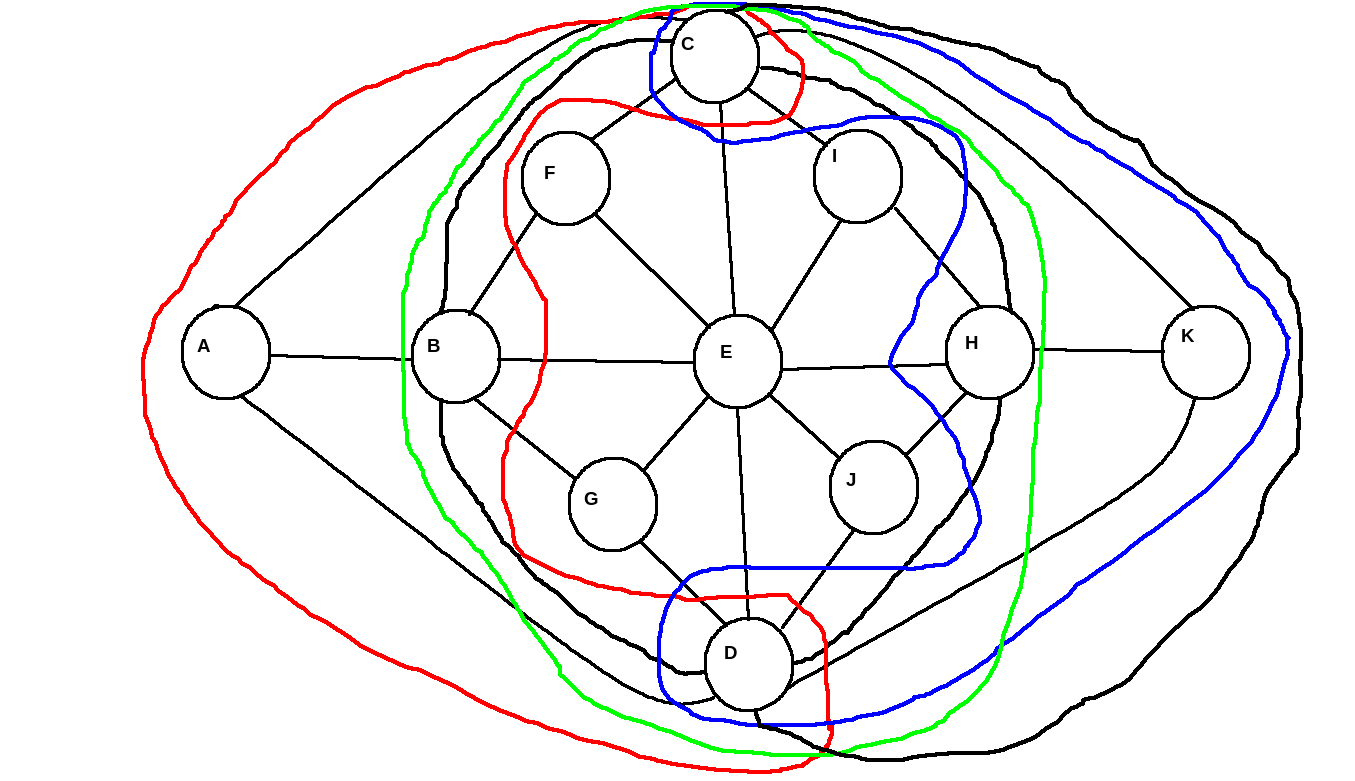
\includegraphics[scale=0.4]{graph_decomp.png}
				\caption{Граф c древесной шириной 3}
				\label{fig:testImage}
		\end{figure}

		\begin{figure}[htbp]
			\centering
				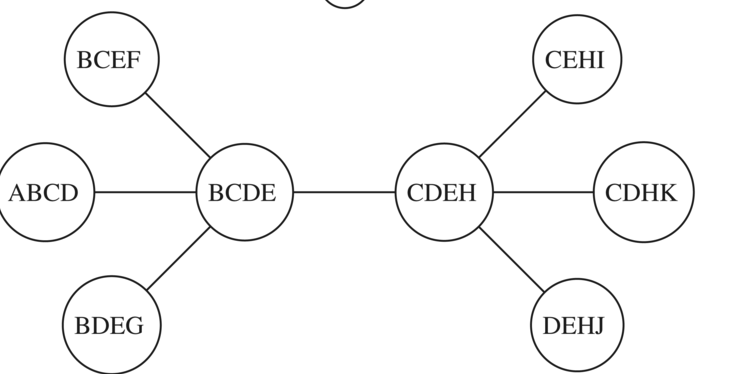
\includegraphics[scale=0.4]{prog_decomp.png}
				\caption{Оптимальная древесная декомпозиция для графа на рисунке 1}
				\label{fig:testImage}
		\end{figure}

		\begin{figure}[htbp]
			\centering
				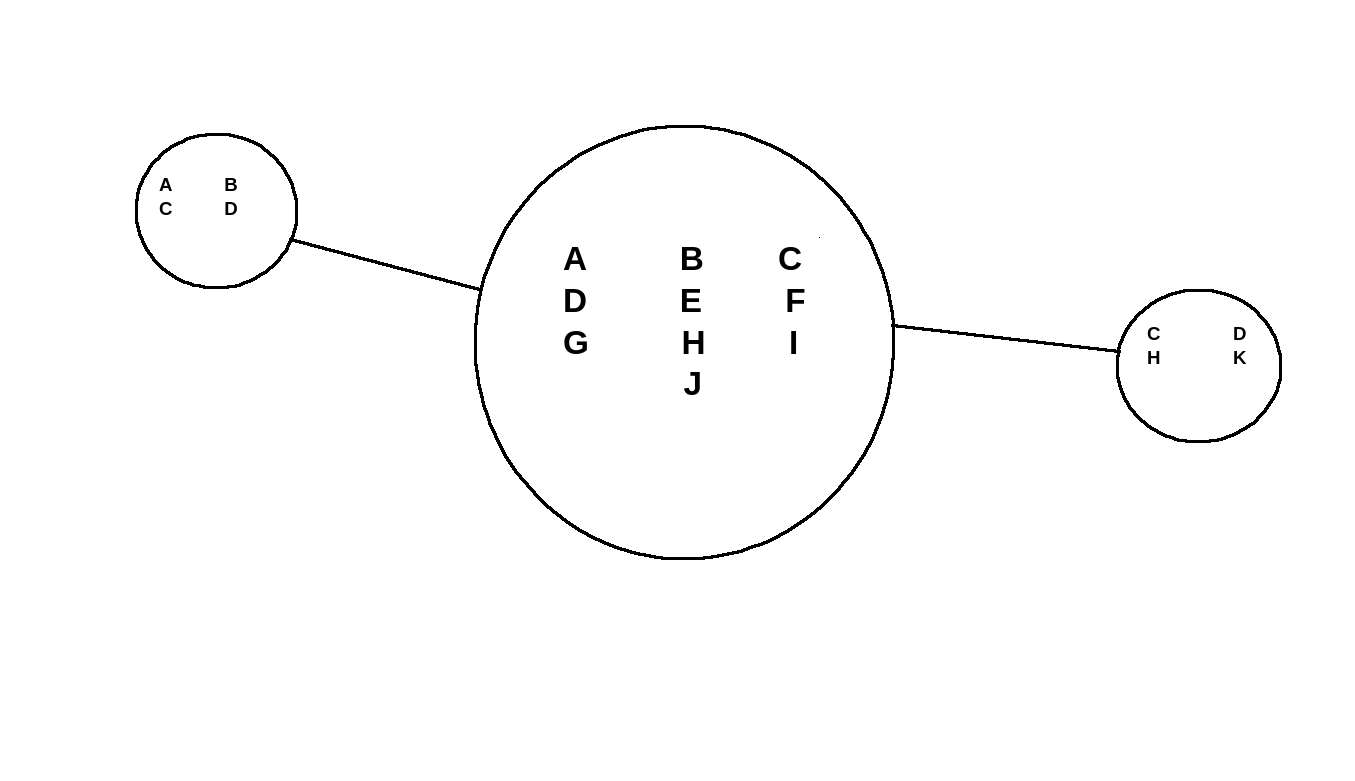
\includegraphics[scale=0.4]{decomp_of_prog.png}
				\caption{Декомпозиция построенная программой для графа на рисунке 1}
				\label{fig:testImage}
		\end{figure}

		Пусть задан граф  $G=(V, E)$, изображенный на рисунке 1. Этот граф называется графом Голднера-Харари и является 3-деревом [18]. 
		Факт того, что этот граф имеет древесную ширину 3 подтверждает рисунок 2 на котором изображена оптимальное древесное разложение.
		На рисунке 3 изображена древесная декомпозиция графа построенная нашим алгоритмом.
		Из-за того, что алгоритм принебрег разложением графа $\{A, B, C, D, E, F, G, H, I, J\}$ из-за того что в нем нет полных подграфов древесная ширина получилась завышенная. Алгоритм дает ответ $9$ вместо $3$.

		Приведем пример неоптимальной оценки работы жадного алгоритма. 
		Пусть $G=(V, E)$, где $V=\{A, B, C, D\}$, $E=\{\{A, B\}, \{A, C\}, \{C, D\}, \{B, D\}\}$. 
		Тогда оптимальное древесное разложение: $\{\{A, B, C\}, \{B, C, D\}\}$.
		А древесное разложение которое было найдено нашим алгоритмом (такая оценка получается из-за отсутствия полных подграфов в графе $G$): $\{A, B, C, D\}$.
		Тогда оценка нашего алгоритма будет равна 3, т.к. не существует полных подграфов в графе $G$, в то время как оптимальная оценка равна 2 $($рис. $4, 5)$.

		Графы на которых тестировалась программа можно разделить на 2 класса: графы протестированные на точность оценки древесной ширины и графы протестированные на время работы программы.
		Сначала приведем графы на которых тестировалась точность оценки и для каждого графа опишем почему эта оценка для него не точна или наоборот, точна.

		\begin{figure}[htbp]
			\centering
				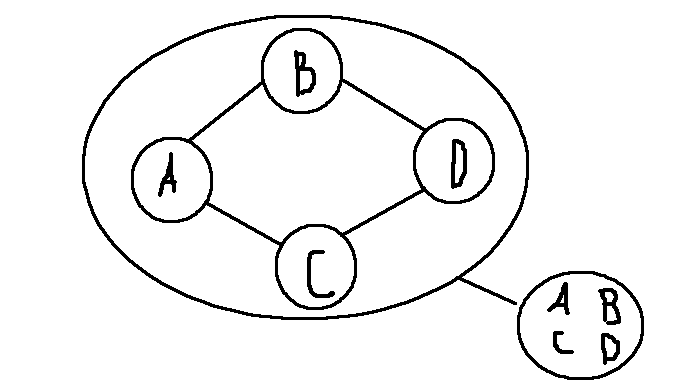
\includegraphics[scale=0.4]{assessmentOfAlg.png}
				\caption{Древесная декомпозиция построенная нашим алгоритмом для графа G}
				\label{fig:testImage}
		\end{figure}

		\begin{figure}[htbp]
			\centering
				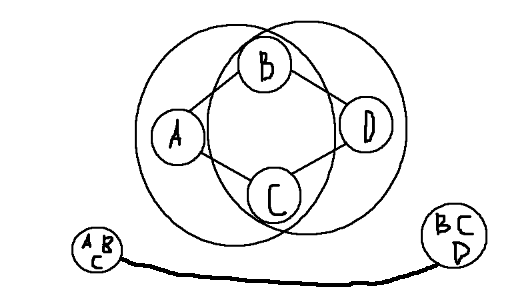
\includegraphics[scale=0.4]{graph_simple_example.png}
				\caption{Древесная декомпозиция с наименьшей шириной.}
				\label{fig:testImage}
		\end{figure}

		Оценим эффективность верхней оценки данного алгоритма на тестах. 

		\begin{table}[]
			\resizebox{\textwidth}{!}{%
			\begin{tabular}{|l|l|l|l|}
			\hline
			Вершины графа & Ребра графа & Оценка алгоритма & Оптимальная оценка \\
			\hline\hline
			$\{A, B, C, D\}$ & $\{\{A, B\}, \{A, C\}, \{B, D\}, \{C, D\}\}$ & 3 & 2  \\
			\hline
			$\{A, B, C, D, E, F, X, Y, Z\}$ & $\{\{A, B\}, \{A, D\}, \{B, C\}, \{B, E\}, \{C, F\}, \{D, E\}, \{E, F\}, \{D, X\}, \{E, Y\}, \{F, Z\}, \{X, Y\}, \{Y, Z\}\}$ & 8 & 2  \\
			\hline
			$\{A, B, C, D, E, F, G, H\}$ & $\{\{A, B\}, \{B, C\}, \{A, C\}, \{C, D\}, \{D, E\}, \{C, E\}, \{B, E\}, \{B, F\}, \{B, G\}, \{F, G\}, \{E, G\}, \{G, H\}, \{E, H\}\}$ & 2 & 2 \\
			\hline
			\end{tabular}%
			}
		\end{table}

		\begin{table}[]
			\resizebox{\textwidth}{!}{%
			\begin{tabular}{|l|l|l|l|}
			\hline
			Вершины графа & Ребра графа & Оценка алгоритма & Оптимальная оценка \\
			\hline\hline
			$\{A, B, C, D, E\}$ & $\{\{A, B\}, \{A, C\}, \{A, D\}, \{A, E\}, \{B, C\}, \{B, D\}, \{B, E\}, \{C, D\}, \{C, E\}, \{D, E\}\}$ & 4 & 4 \\
			\hline
			$\{A, B, C, D, E, F, G, H\}$ & $\{\{A, B\}, \{A, E\}, \{A, H\}, \{B, C\}, \{C, D\}, \{C, G\}, \{D, H\}, \{D, E\},\{E, F\}, \{F, G\}, \{G, H\} \}$ & 7 & 2 \\
			\hline
			$\{A, B, C, D, E, F\}$ & $\{\{A, B\}, \{A, C\}, \{A, E\}, \{A, F\}, \{B, F\}, \{B, D\}, \{B, C\}, \{C, D\}, \{C, E\}, \{D, F\}, \{D, E\}, \{E, F\} \}$ & 5 & 2 \\
			\hline
			\end{tabular}%
		}
		\end{table}

		Здесь, в первой колонке записаны вершины графа на котором проводится тестирование, во второй колонке ребра этого графа, в третьей колонке результат работы алгоритма на данном графе и в четвертой оптимальная оценка этого графа.

		Первый граф из таблицы 1 является простейшим примером неточной оценки древесной ширины нашего алгоритма. Этот пример был показан ранее.
		
		\\
		\\
		\\
		\\
		\\
		\\
		\\
		\\
		\\

		Из таблиц видно, что оценка жадного алгоритма неточная и зависит от количества циклов в графе. 
		К примеру, второй граф из таблицы 1 представляет собой сетку размера 9 $($рис. $6)$.
		Точная оценка древесной ширины этого графа равна 3, но жадный алгоритм дает оценку 9.
		При увеличении размера сетки разность между оптимальной оценкой древесной ширины и оценкой жадного алгоритма будет увеличиватся.

		\begin{figure}[htbp]
			\centering
				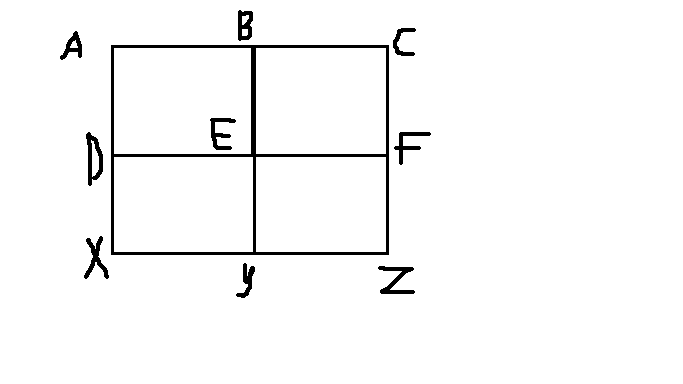
\includegraphics[scale=0.4]{cell.png}
				\caption{Граф-сетка размера 9.}
				\label{fig:testImage}
		\end{figure}

		Третий граф в таблице 1 является примером графа, оцениваемого алгоритмом точно. Это происходит потому, что этот граф состоит из треугольников, т.е. полных графов размера 3.
		Его разложение изображено на рисунке 7.

		\begin{figure}[htbp]
			\centering
				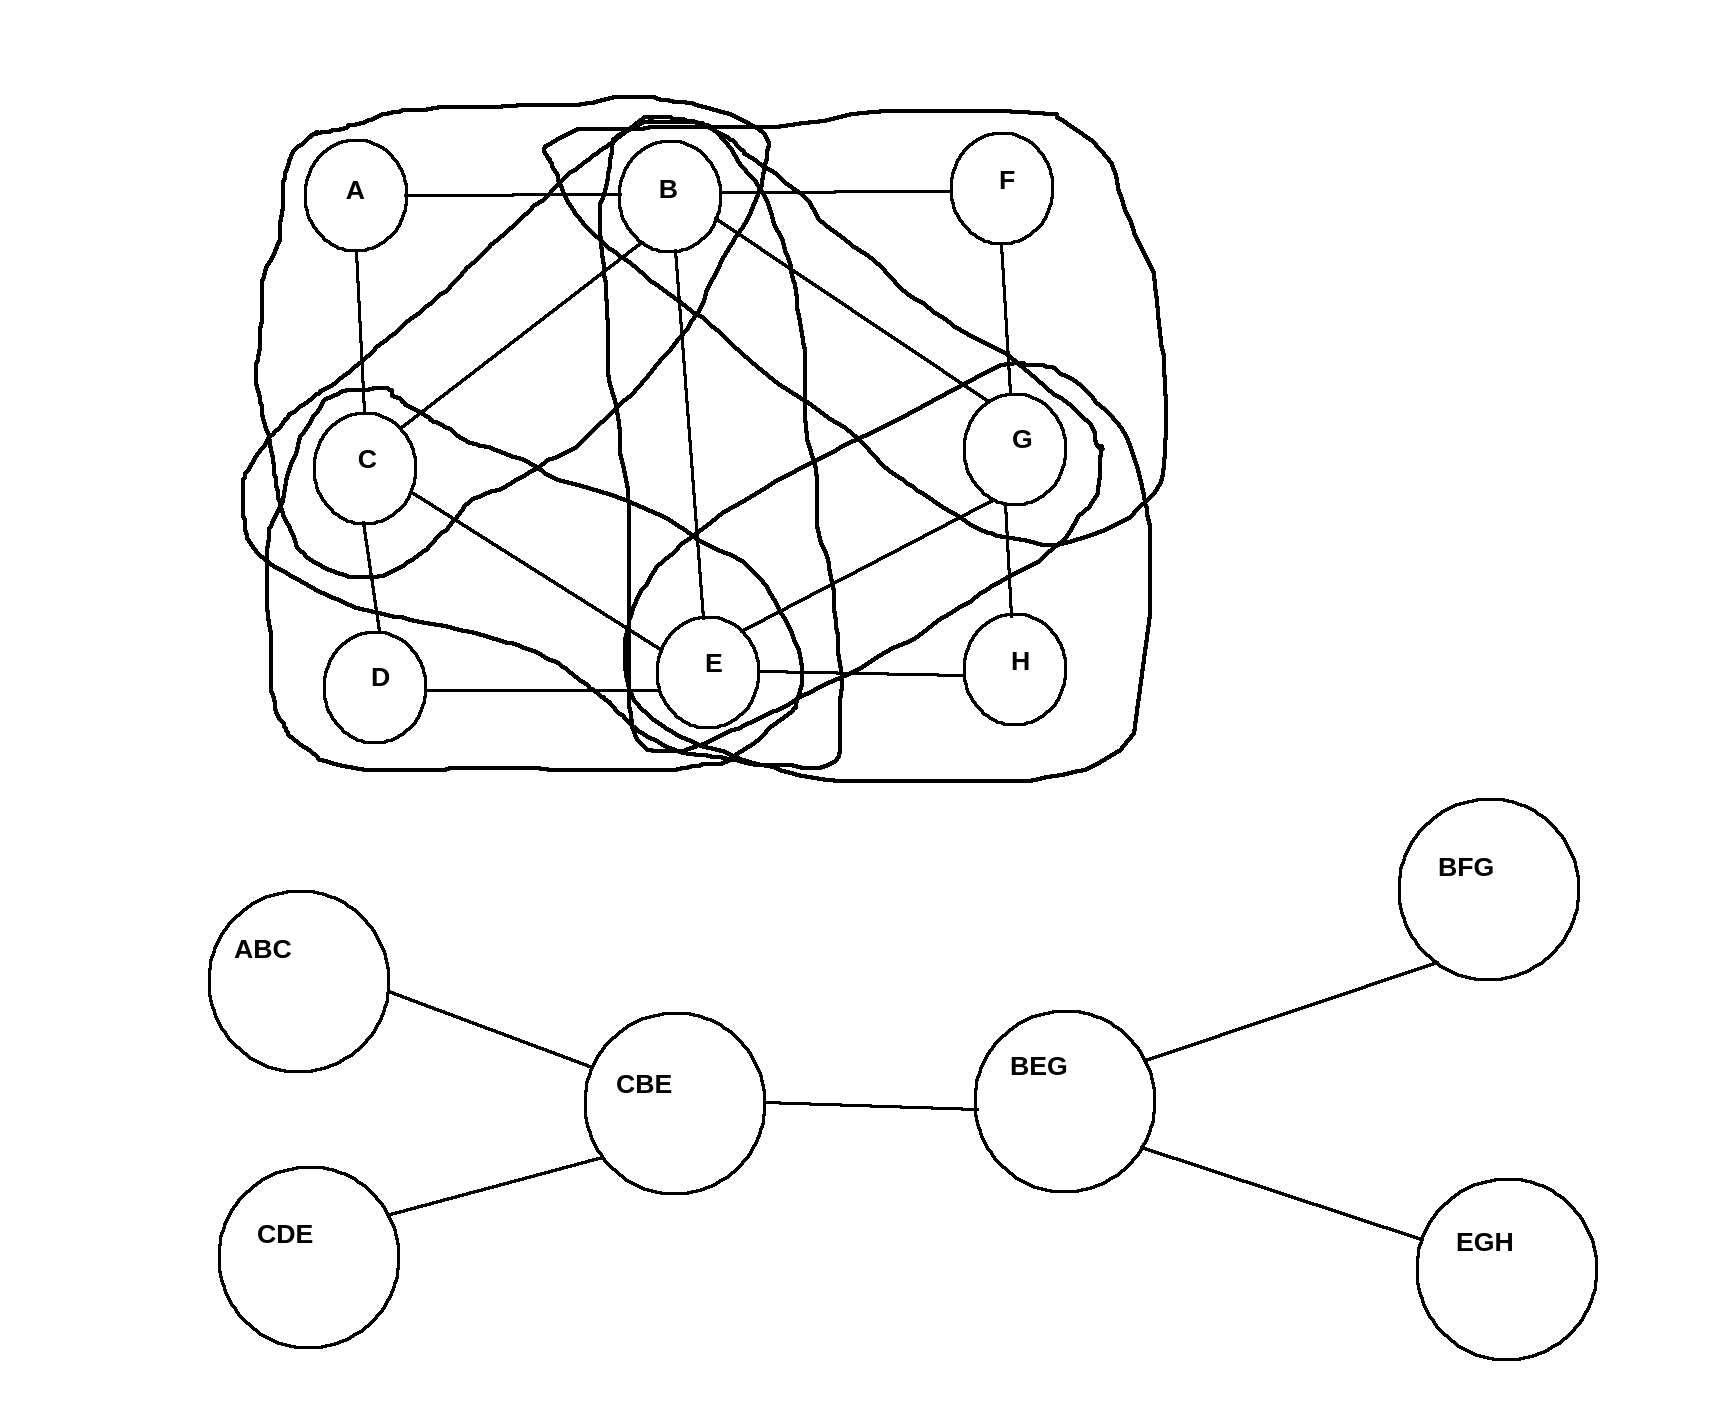
\includegraphics[scale=0.3]{graph3_example.png}
				\caption{Третий граф в таблице 1 и его древесное разложение разложение}
				\label{fig:testImage}
		\end{figure}

		Граф $K_5$ также является отличным примером точной оценки древесной ширины нашим алгоритмом т.к. явлется полным графом (рис. 8).

		\begin{figure}[htbp]
			\centering
				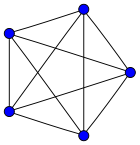
\includegraphics[scale=0.5]{5-vertices_graph.png}
				\caption{полный граф с 5 вершинами}
				\label{fig:testImage}
		\end{figure}

		Второй граф в таблице 2 явлется графом с древесной шириной $2$ из-за соединений всех вершин с тремя другими. Однако из-за того что этот граф не имеет полных подграфов оценка алгоритма является не точной (рис. 9).

		\begin{figure}[htbp]
			\centering
				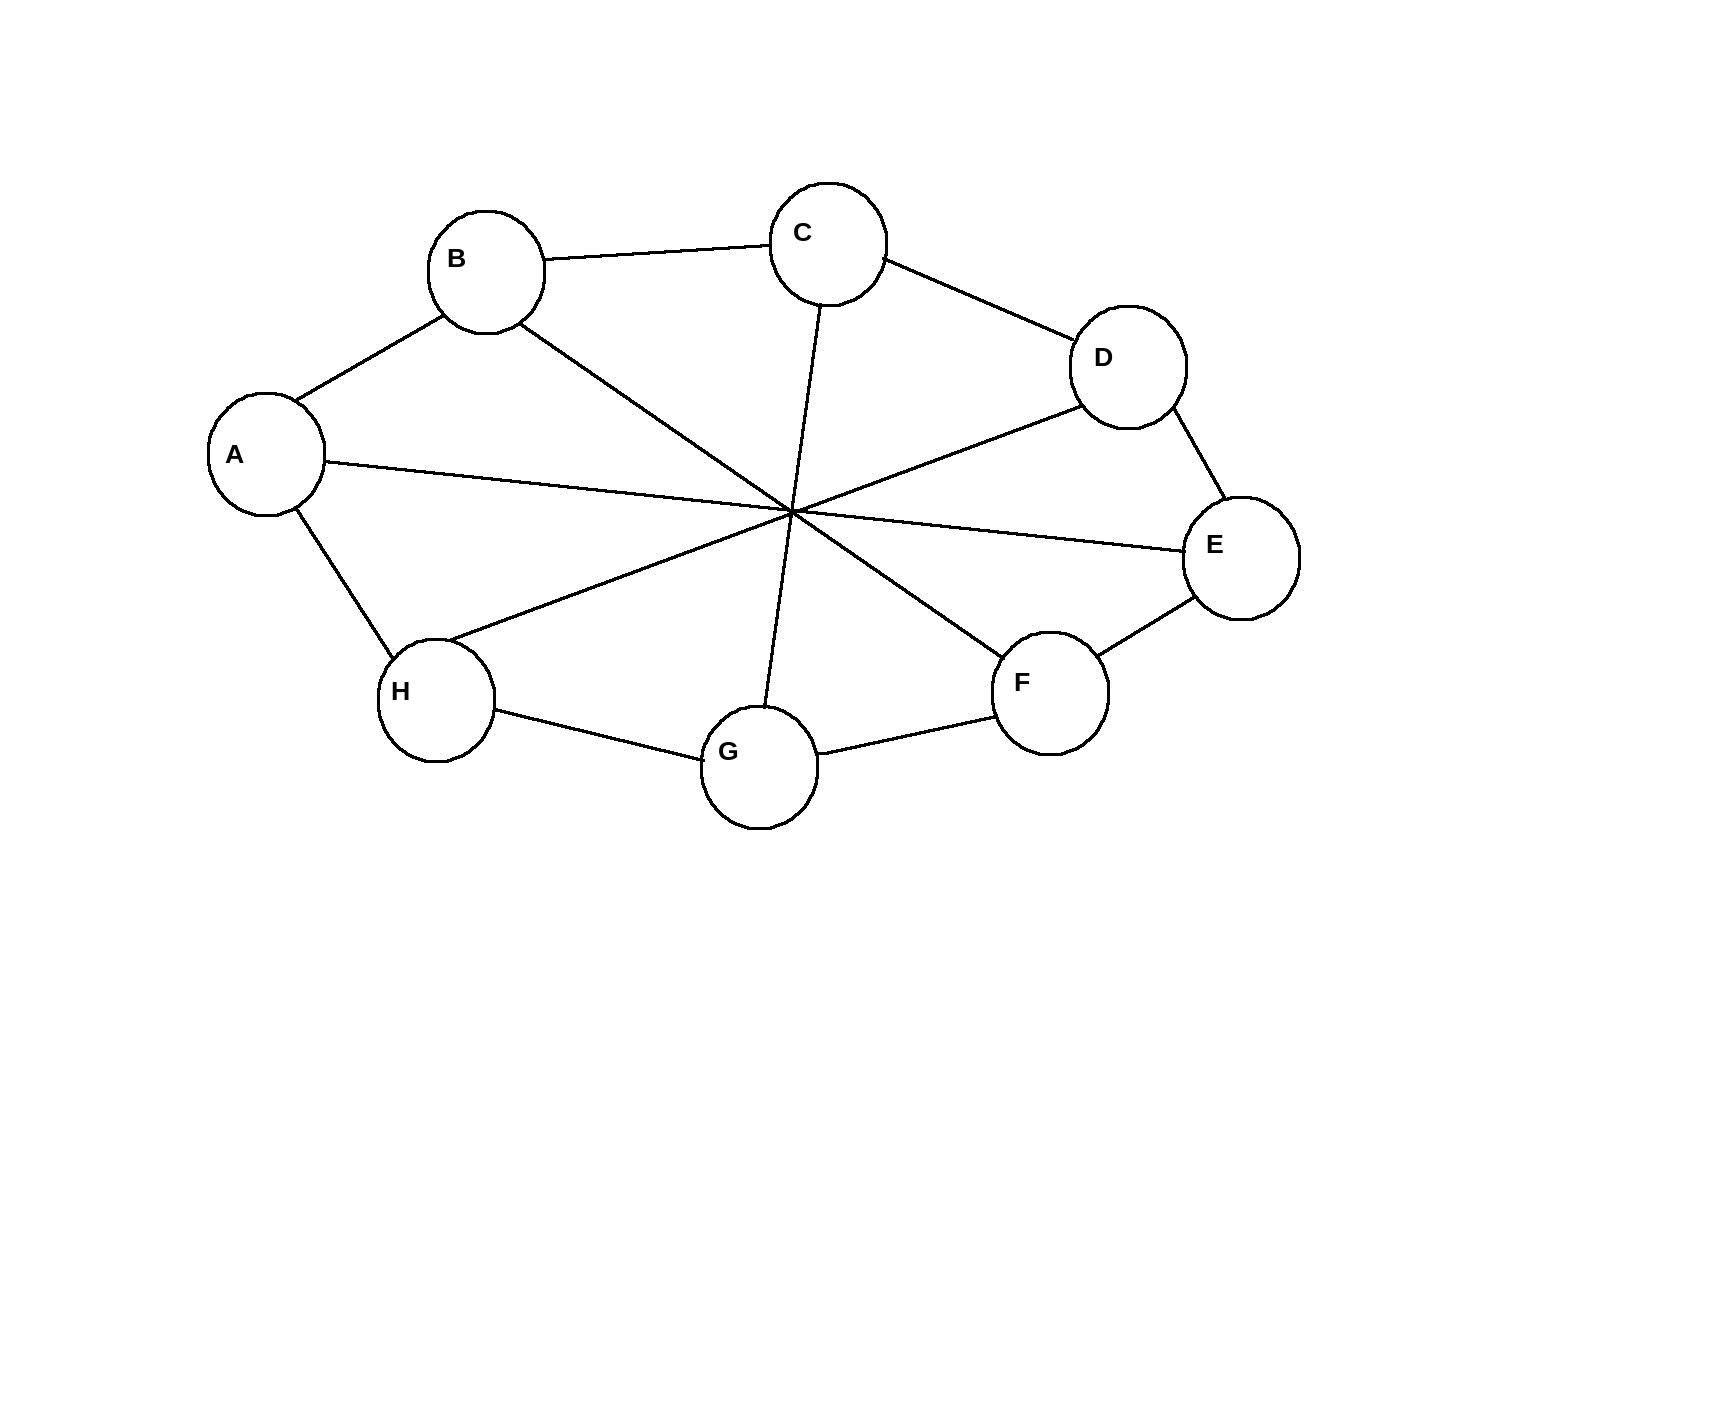
\includegraphics[scale=0.2]{graph_example_cross_out.png}
				\caption{Граф с древесной шириной 3}
				\label{fig:testImage}
		\end{figure}

		Третий граф в таблице 2 называется графом октаэдра и является другим примером графа с древесной шириной $2$. Алгоритм дает оценку $5$ для этого графа (рис. 10).

		\begin{figure}[htbp]
			\centering
				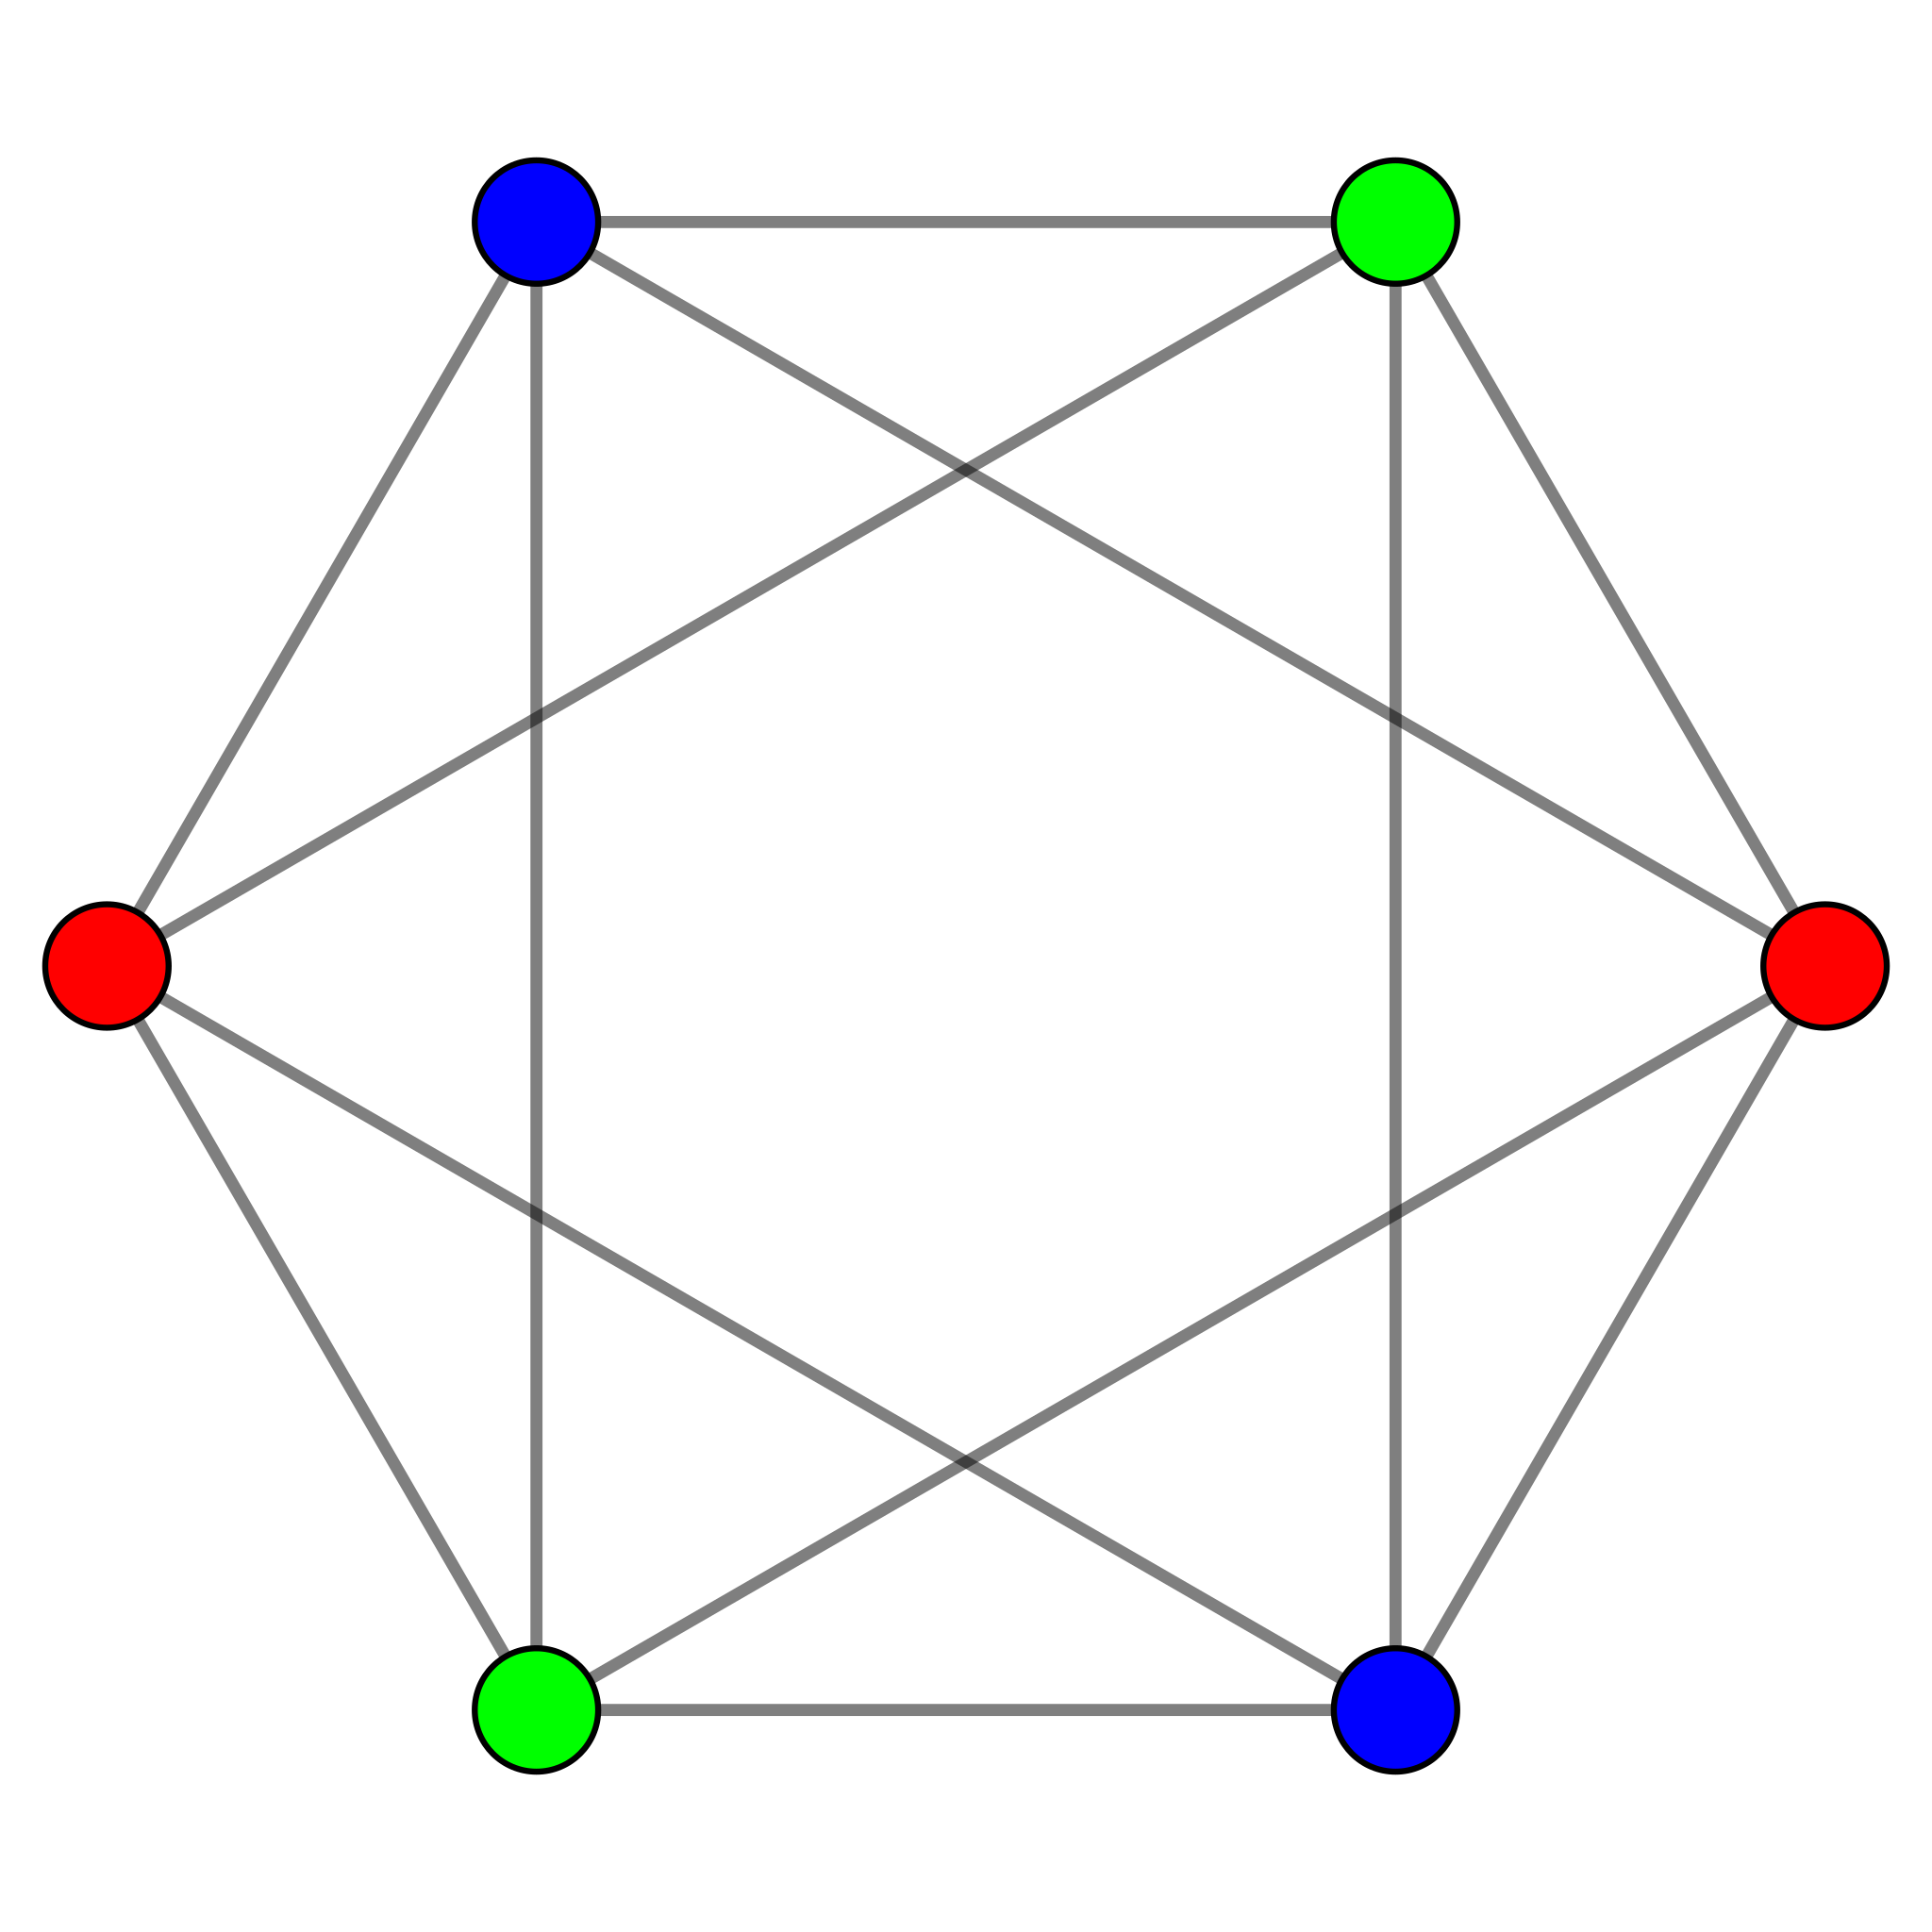
\includegraphics[scale=0.1]{octahedron.png}
				\caption{Октаэдр}
				\label{fig:testImage}
		\end{figure}

		Также стоит отметить, графы с древесной шириной большей $3$ могут быть преобразованы в один из графов из таблицы 2 путем удаления вершин, ребер и стягиванием ребер.

		Проанализируем время работы программы на разном количестве вершин и ребер.

		\begin{table}[]
			\resizebox{\textwidth}{!}{%
			\begin{tabular}{|l|l|l|l|l|}
			\hline
			Количество вершин & Количество ребер & Время в с. & Оценка древесной ширины нашего алгоритма\\
			\hline\hline
			100 & 32 & 0.67 & 1 \\
			\hline
			100 & 57 & 0.76 & 1 \\
			\hline
			100 & 63 & 0.7 & 9 \\
			\hline
			100 & 155 & 0.18 & 82 \\
			\hline
			100 & 166 & 0.21 & 81 \\
			\hline
			100 & 281 & 0.11 & 99 \\
			\hline
			100 & 2395 & 0.36 & 99 \\
			\hline
			100 & 2422 & 0.37 & 99 \\
			\hline
			100 & 2434 & 0.43 & 99 \\
			\hline
			100 & 2485 & 0.37 & 99 \\
			\hline
			100 & 2483 & 0.42 & 99 \\
			\hline
			100 & 2488 & 0.4 & 99 \\
			\hline
			100 & 2489 & 0.37 & 99 \\
			\hline
			100 & 2511 & 0.38 & 99 \\
			\hline
			200 & 96 & 7.98 & 1 \\
			\hline
			200 & 219 & 5.85 & 112 \\
			\hline
			200 & 226 & 4.62 & 125 \\
			\hline
			200 & 9846 & 3.85 & 199 \\
			\hline
			200 & 9901 & 3.81 & 199 \\
			\hline
			200 & 9907 & 4.23 & 199 \\
			\hline
			200 & 9922 & 4.86 & 199 \\
			\hline
			200 & 9938 & 4.32 & 199 \\
			\hline
			200 & 9940 & 3.87 & 199 \\
			\hline
			200 & 9968 & 4.14 & 199 \\
			\hline
			200 & 10016 & 4 & 199 \\
			\hline
			\end{tabular}%
		}
		\end{table}

		\begin{table}[]
			\resizebox{\textwidth}{!}{%
			\begin{tabular}{|l|l|l|l|}
			\hline
			Количество вершин & Количество ребер & Время в с. & Оценка древесной ширины нашего алгоритма\\
			\hline
			300 & 435 & 13.78 & 218 \\
			\hline
			300 & 449 & 16.46 & 213 \\
			\hline
			300 & 490 & 7.5 & 254 \\
			\hline
			300 & 927 & 1.93 & 296 \\
			\hline
			300 & 22249 & 16.95 & 299 \\
			\hline
			300 & 22358 & 18.76 & 299 \\
			\hline
			300 & 22363 & 18.59 & 299 \\
			\hline
			300 & 22366 & 16.98 & 299 \\
			\hline
			300 & 22414 & 19.09 & 299 \\
			\hline
			300 & 22486 & 18.98 & 299 \\
			\hline
			300 & 22454 & 19.25 & 299 \\
			\hline
			300 & 22513 & 19.39 & 299 \\
			\hline
			400 & 387 & 95.13 & 187 \\
			\hline
			400 & 420 & 96.39 & 194 \\
			\hline
			400 & 815 & 12.93 & 358 \\
			\hline
			400 & 1527 & 5.22 & 397 \\
			\hline
			400 & 4011 & 9.6 & 399 \\
			\hline
			400 & 39746 & 57.36 & 399 \\
			\hline
			400 & 39915 & 57.02 & 399 \\
			\hline
			400 & 40027 & 65.25 & 399 \\
			\hline
			400 & 40140 & 56.37 & 399 \\
			\hline
			400 & 388 & 98.51 & 169 \\
			\hline
			500 & 611 & 137.07 & 323 \\
			\hline
			500 & 1246 & 13.73 & 476 \\
			\hline
			500 & 1324 & 10.67 & 483 \\
			\hline
			500 & 3724 & 12.46 & 499 \\
			\hline
			500 & 62328 & 134.82 & 499 \\
			\hline
			500 & 6292 & 19.56 & 499 \\
			\hline
			500 & 62328 & 134.82 & 499 \\
			\hline
			\end{tabular}%
		}
		
		\end{table}


		\begin{table}[]
		\resizebox{\textwidth}{!}{%
		\begin{tabular}{|l|l|l|l|}
		\hline
		Количество вершин & Количество ребер & Время в с. & Оценка древесной ширины нашего алгоритма \\
		\hline
		600 & 173 & 461.04 & 1 \\
		\hline
		600 & 1768 & 16.79 & 585 \\
		\hline
		600 & 8997 & 36.412 & 599 \\
		\hline
		600 & 89865 & 292.81 & 599 \\
		\hline
		700 & 272 & 920.31 & 2 \\
		\hline
		700 & 2492 & 26.19 & 695 \\
		\hline
		700 & 12244 & 64.28 & 699 \\
		\hline
		700 & 122473 & 541.60 & 699 \\
		\hline
		800 & 317 & 1484.20 & 1 \\
		\hline
		800 & 3196 & 37.71 & 797 \\
		\hline
		800 & 15875 & 98.95 & 799 \\
		\hline
		800 & 159547 & 820.11 & 799\\
		\hline
			\end{tabular}%
			}
	
		\end{table}

		\begin{figure}[htbp]
			\centering
				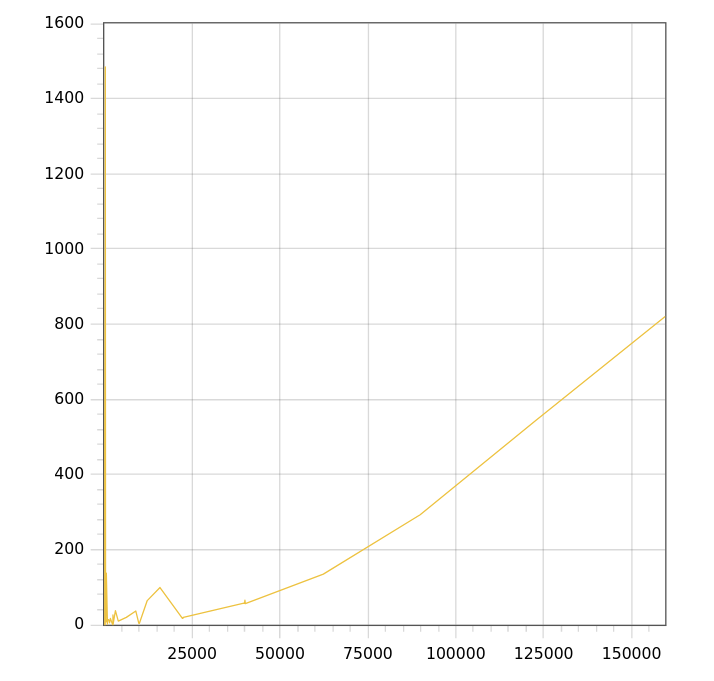
\includegraphics[scale=0.4]{graph_time.png}
				\caption{График времени работы программы}
				\label{fig:testImage}
		\end{figure}

		Минимальное значение рёбер в графе $G$ на котором достигается максимальное значение древесной ширины назовём пороговым значением по древесной ширине на данном графе.
		Графы из таблиц были получены случайной генерацией на вершинах количеством в интервале от 100 до 800 с шагом 100 и количеством ребер в них, составляющим от 0.1 до 50 процентов от количества ребер в полном графе на этих вершинах, в зависимости от того, является ли данное значение пороговым по древесной ширине на соответствующем графе (к примеру для графа на 100 вершинах пороговым значением древесной ширины является 99).

		В таблицах, в первых двух столбцах записано количество вершин и количество рёбер в генерируемых графах. В третьем столбце записано время работы алгоритма на этих графах. В четвертом столбце записана древесная ширина для этих графов.

		В таблицах видно, что с увеличением количества вершин увеличивается время затрачиваемое на исполнение программы.
		Из количества вложенных циклов в алгоритме видно что, алгоритм имеет ассимптотику $O(n \cdot m+n^2 \cdot m+n^2)$, где $n$ --- количество вершин в графе $G$,  $m$ --- количество ребер в графе $G$.
		Здесь за $O(n \cdot m)$ выделяем подграф, образуемый вершиной вместе с ее смежными вершинами, за $O(n^2 \cdot m)$ удаляем подграф из стартового графа, за $O(n^2)$ проверяем является ли выделенный подграф полным.
		В этой ассимптотике можно убедится, просмотрев код программы в приложении.
		В таблице также видно, что малое количество рёбер при большем количестве вершин также приводит к увеличению времени работы программы.

		На графике, изображенном на рисунке 11, горизотальная ось означает количество рёбер, вертикальная ось - время, затраченное на работу программы на графе с данным количеством рёбер.
		Здесь видно, что при увеличении количества рёбер время затраченное на работу программы увеличивается. Также на графике видно, что большое количество вершин и малое количество рёбер приводит к большому времени работы программы.

		\end{large}
		\newpage
		\\
		\\
		\\
		\section{Заключение}
		\renewcommand{\baselinestretch}{1.5}
		
		Был рассмотен жадный алгоритм верхней оценки древесной ширины, основанный на выделении полных подграфов из входного графа.

		Можно заключить, что программа имеет время работы соответствующее ряду $O(n \cdot m+n^2 \cdot m+n^2)$, причем время зависит от количества ребер в графе.
		
		Алгоритм дает верхнюю, а не точную оценку древесной ширины. Также было изложено предположение, что верхняя оценка древесной ширины, зависит от количества циклов, имеющихся в графе, что исходит из того, что алгоритм основан на выделении из графа полных подграфов, а не k-деревьев. 
		А следовательно, с ростом числа циклов, оценка жадного алгоритма верхней оценки древесной ширины становится менее точной.

		Графы оцениваемые алгоритмом точно являются либо полными, либо графами из которых можно выделить полные подграфы.

		\newpage
		\renewcommand{\baselinestretch}{1.5}

		\begin{thebibliography}{100}
			%references

			\bibitem{BHP} Bodlaender H.L. A partial k-arboretum of graphs with bounded treewidth // Theoretical Computer Science. 1998. V. 209, N 2--3. P. 1--45.

			\bibitem{AP} Arnborg S., Proskurowski A. Linear time algorithms for NP-hard problems restricted to partial k-trees // Discrete Applied Mathematics. 1989. V. 23, N 1. P. 11--24.

			\bibitem{BL} Bern M.W., Lawler E.L., Wong A.L. Linear-time computation of optimal subgraphs of decomposable graphs // Journal of Algorithms. 1987. V. 8, N 2. P. 216--235.

			\bibitem{BHD} Bodlaender H.L. Dynamic programming on graphs with bounded treewidth // International Colloquium on Automata, Languages, and Programming. 1988. V. 317, N 15. P. 105-118.

			\bibitem{ADPC} Arnborg S., Derek G.C., Proskurowski A. Complexity of Finding Embeddings in a k-Tree // SIAM Journal on Algebraic Discrete Methods. 1987. V. 8 P. 277--284.

			\bibitem{BHLA} Bodlaender H.L. A linear time algorithm for Finding tree-decompositions of small treewidth // SIAM Journal on Computing. 1996. V. 25, N 6. P. 226--234.

			\bibitem{SMP} Syslo M.M., Proskurowski A. On Halin graphs // Lecture Notes in Mathematics. 1983. V. 1018. P. 248--256.

			\bibitem{ACP} Arnborg S., Corneil G.D., Proskurowski A. Complexity of Finding embeddings in a k-tree // SIAM Journal on Matrix Analysis and Applications. 1987. V. 8. P. 277--284.

			\bibitem{RSP} Robertson N., Seymour P.D. Graph Minors XIII: The Disjoint Paths Problem // Journal of Combinatorial Theory. 1995. V. 63, N 1. P. 65--110.

			\bibitem{BHL} Bodlaender H.L. A linear time algorithm for Finding tree-decompositions of small treewidth // SIAM Journal on Computing. 1996. V. 25, N 6. P. 226--234.

			\bibitem{FHL} Feige U., Mohammad H.T., Lee J.R. Improved approximation algorithms for minimum-weight vertex separators // SIAM Journal on Computing. 2008. V. 38, N 2. P. 629--657.

			\bibitem{JR} Matoušek J., Thomas R. Algorithms finding tree-decompositions of graphs // Journal of Algorithms. 1991. V. 12. P. 1--22.

			\bibitem{CRP} Arnborg S., Proskurowski A. Characterization Recognition of Partial 3-Trees // SIAM Journal on Algebraic Discrete Methods. 1986. V. 7. P. 305--314.

			\bibitem{CFE} Bondy J.A., Murty U.S.R. Graph theory with applications. Ontario: Springer London, 2008.

			\bibitem{CRPS} Емеличев В.А., Мельников О.И., Тышкевич Р.И. Лекции по теории графов. Москва: Наука, 1990.

			\bibitem{WPB} Hlinen P., Oum S., Seese D., Gottlob G. Width Parameters beyond tree-width and their applications // The Computer Journal. 2008. V. 51, N 3. P. 326--362.

			\bibitem{OR} Электронный ресурс: https://github.com/ghost171/AlgorithmOfFindingTreeWidth

			\bibitem{WPB} Goldner A., Harary F. Note on a smallest nonhamiltonian maximal planar graph // Bull. Malaysian Math. Soc. 1975. V. 6, N 1. P. 41--42.

		\end{thebibliography}
		
		\newpage
		\section{Приложение}
		\renewcommand{\baselinestretch}{1.5}

		Код программы на языке python также можно просмотреть на github: 
		
		https://github.com/ghost171/AlgorithmOfFindingTreeWidth

		Напишем для начала функцию определяющую является ли поданный аргументом граф полным.
		
		\begin{algorithm}
			\caption{Функция для проверки графа, на полноту}\label{Функция}
			\begin{algorithmic}[1]
			  	\Procedure{IsItClique}{$gr$}
					\State $i \gets 0$
				  	\State $answers \gets []$
				  	\For{\texttt{x in gr.values()}}
					  	\If{$len(x) = len(gr.keys())$}
							\State $answers[i] \gets 1$
					  	\Else
							\State $answers[i] \gets 0$
					  	\EndIf
					  	\State $i \gets i+1$
					\EndFor
		
				  	\For{\texttt{answer in answers}}
						\If{answer = 0}
							\Return 0
					  	\EndIf
				  	\EndFor
		
				  	\Return 1
				\EndProcedure
		\end{algorithmic}
		\end{algorithm}


		Напишем теперь алгоритм нахождения древесной ширины. Дан граф $G$ представляемый списком смежности. Требуется вернуть древесную ширину этого графа.

		\begin{algorithm}[tbp]\footnotesize
			\caption{Жадный алгоритм нахождения древесной ширины}\label{Жадный алгоритм}
			\begin{algorithmic}[2]
				
				\If{\texttt{$IsItClique(graph) = 1$}}
					\State $graph \gets len(graph.keys()) - 1$
					\Return $treewidth$
				\EndIf
				
				\COMMENT{Будем перебирать все вершины начиная с вершин с наименьшей степенью и искать клики}

				\State $lengths \gets []$ 

				\For{\texttt{i, x in enumerate(graph.items())}}
					lengths[i] = (x[0], len(x[1]))
				\EndFor

				$Sort(lengths, 1)$ \COMMENT{Сортируем массив lengths по первому аргументу}

				\State $HGraph \gets graph$

				\While{true}
          			\State $sizeOfTreeDecomposition \gets sizeOfTreeDecomposition + 1$
          			\If{$IsItClique(HGraph)$}
              			\State $s.append(list(HGraph.keys()))$
              			\State $n \gets sizeOfTreeDecomposition$
              			\State $break$
          			\Else
              			\State $vI \gets "a"$
              			\State $adjacentEdgeOfVI \gets []$
              			\For{$\texttt{letter, x in lengths}$}
                  			\State $adjustedVertices \gets []$
                  			\If{letter in HGraph.keys()}
								\For{$\texttt{adj in HGraph[letter]}$}
									adjustedVertices.append(adj)
								\EndFor
                  			\EndIf
                  			\State $adjustedVertices.append(letter)$
                  			\State $graphCopy \gets HGraph$
                  			\State $keys \gets graphCopy.copy().keys()$

                  			\For{$\texttt{key in keys}$}
                      		\If{\texttt{key not in AdjustedVertices}}
                          		\State \texttt{del GraphCopy}
                          		\For{\texttt{x in graphCopy.keys()}}
                            		\If{keyInGraphCopy[x]}
                                  		\State $graphCopy[x].remove(key)$
                              		\EndIf
                          		\EndFor
                      		\EndIf
		\end{algorithmic}
			\end{algorithm}	
			\begin{algorithm}[tbp]\footnotesize
				\caption{Жадный алгоритм нахождения древесной ширины}\label{Жадный алгоритм}
				\begin{algorithmic}[2]
                  			\If{\texttt{len(graphCopy) != 0 \textbf{And} IsItClique(graphCopy)}} 
                      			\State $vI \gets letter$
                      			\State $adjacentEdgeOfVI \gets graphCopy[vI]$
                      			\State $findClique \gets 1$
                      			\State $break$
                  			\EndIf
              			\EndFor
						\If{\texttt{findClique = 0}}
							\State $s.append(HGraph.keys())$
							\State $break$
						\EndIf
						\State $adjacentEdgeOfVI.append(vI)$
						\State $s.append(adjacentEdgeOfVI)$
						\If{\texttt{$len(adjacentEdgeOfVI) > treeWidth$}}
							\State $treeWidth = len(adjacentEdgeOfVI)$
						\EndIf
              			\State \texttt{del HGraph[vI]}

						\For{\texttt{x in HGraph.keys()}}
							\If{\texttt{$vIInHGraph[x]$}}
								\State $HGraph[x].remove(vI)$
							\EndIf
						\EndFor

						\If{\texttt{$len(HGraph.keys()) = 0$}}
							\State $break$
						\EndIf
					\EndIf
				\EndWhile
				\For{el in s}
          			\If{\texttt{len(el) < minEl \textbf{or} minEl = 0}}
              			\State $minEl \gets len(el)$
          			\EndIf
      			\EndFor \\
      			\Return minEl
			\end{algorithmic}
		\end{algorithm}

\end{document}